\section{Resultados}
La configuración inicial que se le dio a cada sistema esta dado por las siguientes ecuaciones:
\begin{align*}
    x_{i+1}&=(i-1)*0.9+a\\
    y_{i+1}&=\left\lbrace\begin{matrix}
        0.5+a & mod(i,2)=0 \\
        a & mod(i,2)\neq 0
    \end{matrix} \right.
\end{align*}
donde a representa un número aleatorio entre -0.1 y 0.1. Con ello, las configuraciones iniciales de cada ejecución del modelo estan
mostradas en la figura \ref{fig:posini}.
\begin{figure}[H]
    \centering
    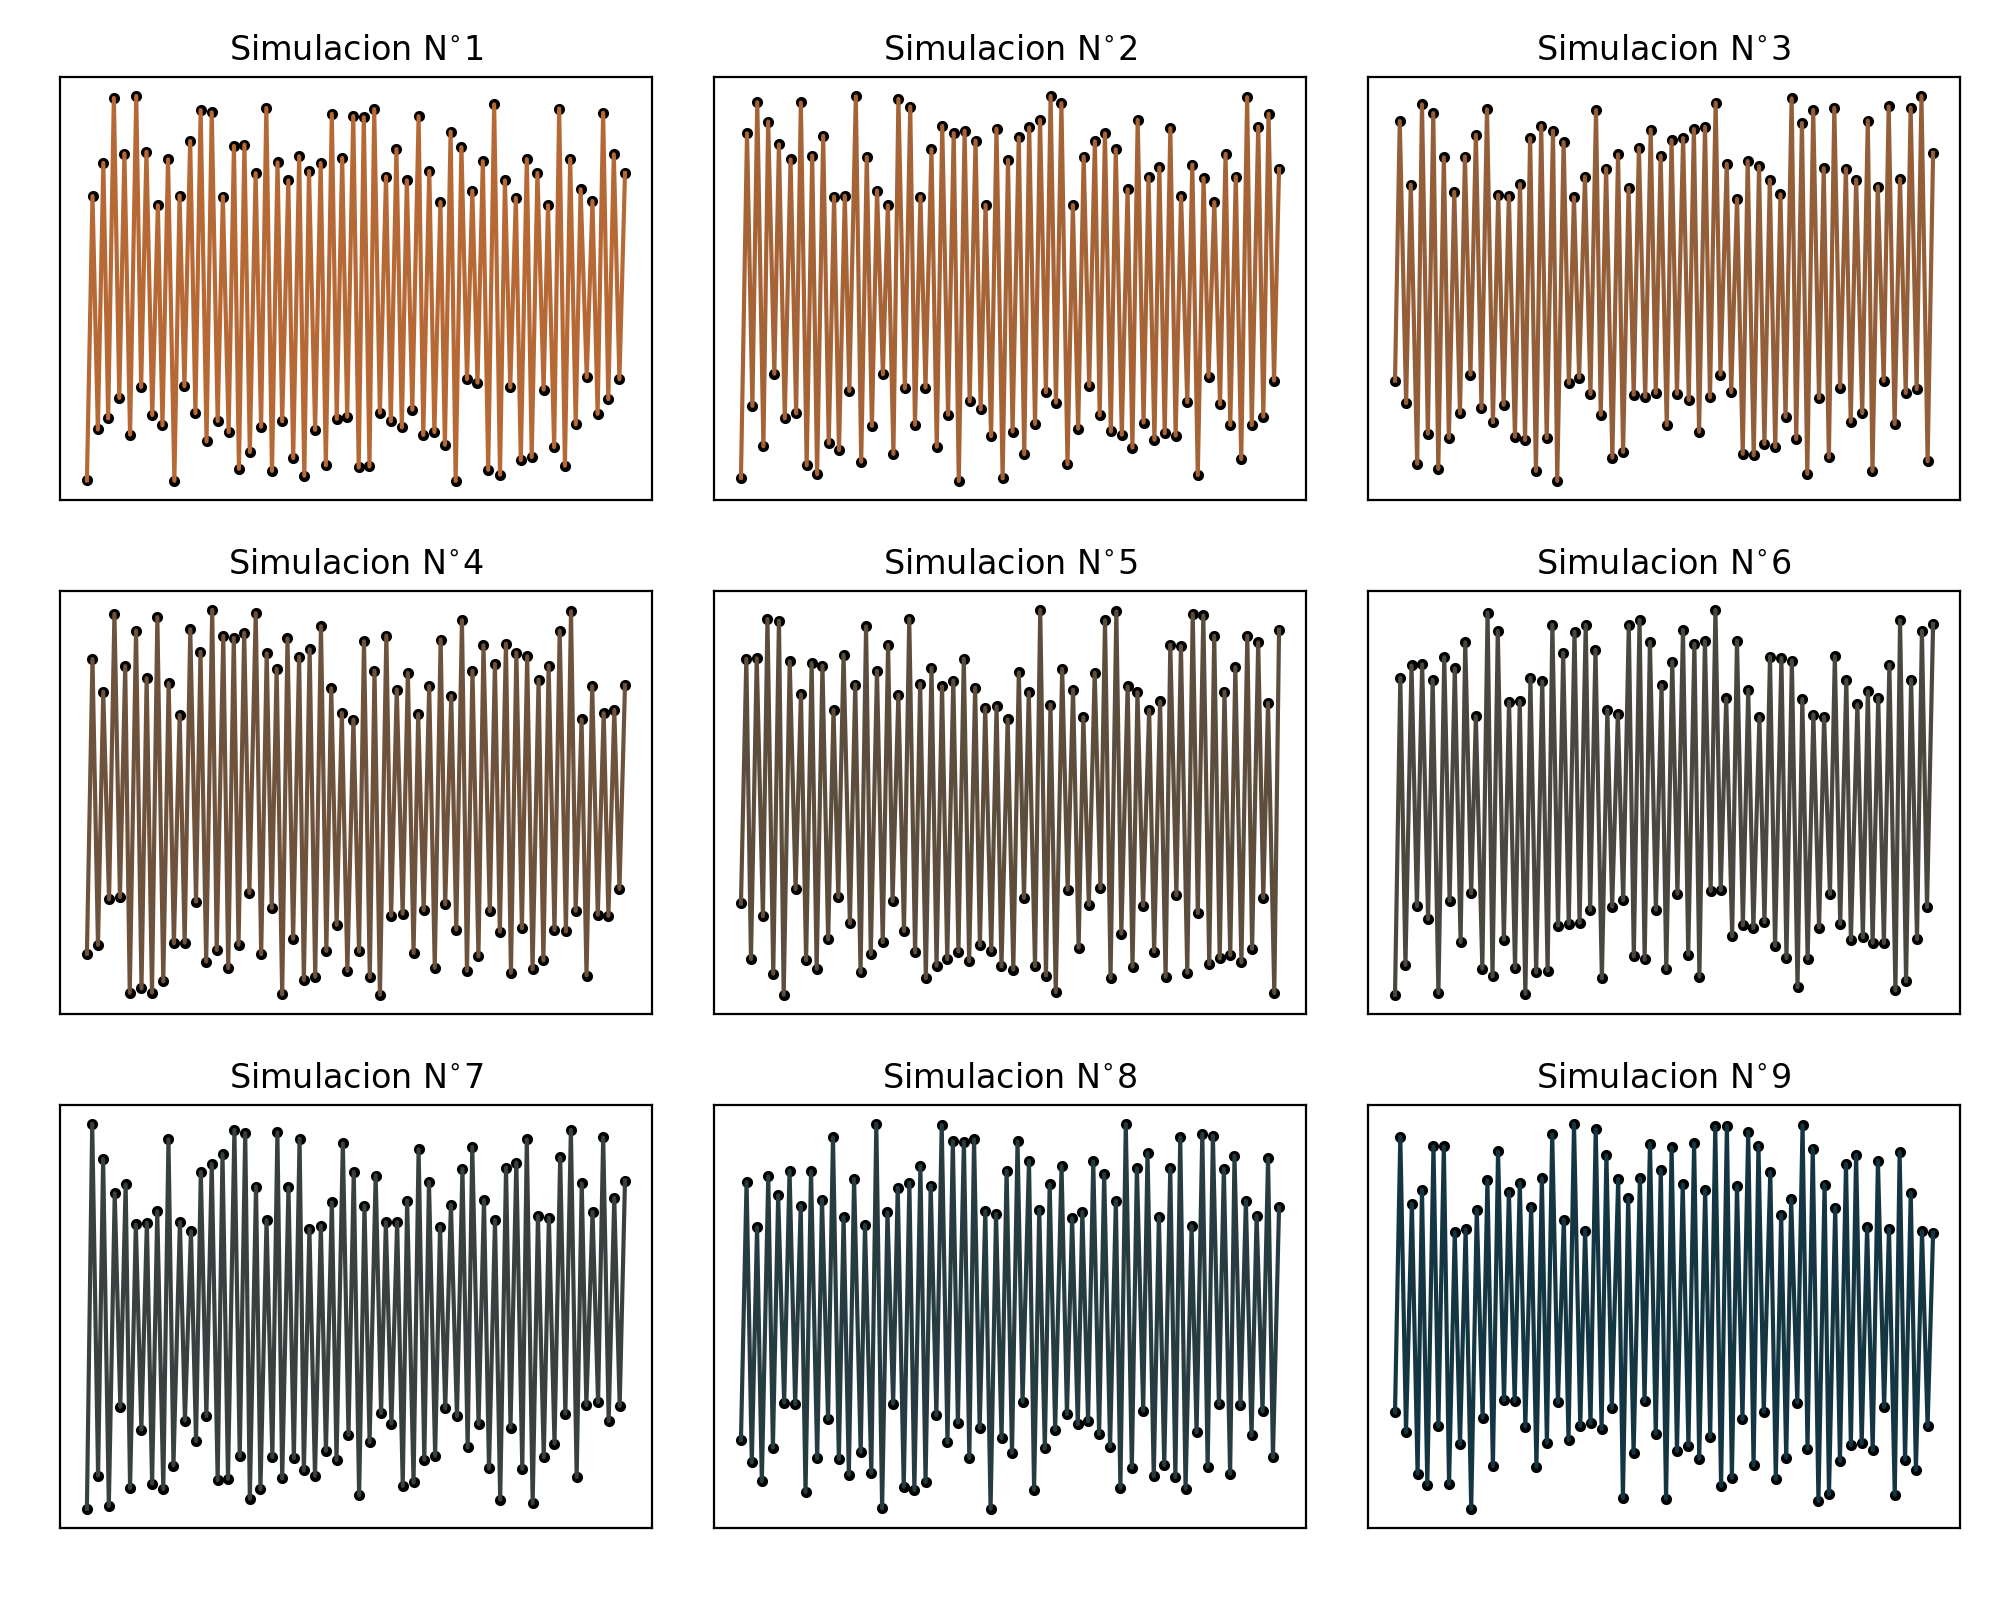
\includegraphics[scale=0.27]{../Graphics/pos_ini.png}
    \caption{Configuración inicial de las cadenas de moleculas.}
    \label{fig:posini}
\end{figure}
Las velocidades de cada molecula fueron dada siguiendo las siguientes ecuaciones:
\begin{align*}
    v_{xi}&=v_{0}\cos(2v_0\pi)\\
    v_{yi}&=v_{0}\sin(2v_0\pi)\\
\end{align*}
donde $v_0$ es un número aleatorio entre 0 y 1. Los parámetros usados para cada simulación son los que se muestran en la tabla \ref{table:parametros},
la dinámica que presento cada simulación estan guardadas en el siguiente link